\section{Contact Database and User Recordings}
\subsection{Overview}
The contact database stores known acoustic signatures allowing you to build a library of known contacts, and to compare current contacts with those in the database. The database is stored in a single file called \path{sonar.db} in the MACS application data folder. The database is created automatically when MACS is first run, and is empty until you add your own contacts. Further details about the fields and structure of the database are discussed in Appendix C. MACS also allows you to record contacts and store them in the database. The recordings are stored in a separate folder, which is set in the \textbf{Settings} panel.

\begin{faintquote}
    This section provides a basic outline of the process and workflow for contact recording and matching. A more detailed process workflow is given in the Illustrated Examples section.
\end{faintquote}

\subsubsection{Installing the pre-populated database}
If you wish you can install a pre-populated database of known contacts. At the time of writing this database contains all of the vessels included in the MNW Recognition Guide, excluding aircraft, and is intended to be a starting point for your own database. As such it does not contain the LOFARgram details. It is assumed that users would prefer to update the database with their own recordings. To install the database:

\begin{compactenum}
    \item Download the \href{https://github.com/Mahzel/MACS}{MNW Defaults} database file from the MACS website.
    \item \verb|MNW_Defaults.db| will download to users Download folder
    \item Open MACS
    \item In the right panel select Import from the Contacts subpanel
    \item Follow on screen direction to install the prepopulated database
\end{compactenum}

\subsection{Contact Database}
\subsubsection{Terminology}
\begin{compactitem}
    \item Contact: A hull with defined constants e.g. name, propulsion type, nationality etc.
    \item Measurement: An observation made with the tools, attached to a contact. A single contact can have multiple measurements.
    \item Recording: A sound file containing a contact's acoustic signature. %Recordings are linked
\end{compactitem}

\subsubsection{Database Interface}
The database and recordings management panels are on the right side of the application window Figure 6. The right side panels can be hidden by clicking the right pointing arrow and the sub-panels can be collapsed to save space. The database panel has the following sub-panels:

\begin{compactitem}
    \item Compare against database: Shows a list of all contacts in the database which match your marked frequencies.
    \item Marked frequencies:
    \item New contact: Allows you to add a new contact to the database.
    \item Contacts: Browse, import and export contacts.
\end{compactitem}

The recordings panel shows a list of all recordings in the recordings folder, and allows you to add, rename and delete recordings.

To add a recording to the database first make sure that the in-game sound is being captured by MACS. Then click the \enquote{\textbf{REC}} button on the applications Top Tool Bar. You should capture a recording of sufficient length to ensure that you have captured a full range of sounds. On playback the recording can be looped so that it appears continuous when you are performing an analysis. The panel allows an adjustment of playback speed which is very useful when you are trying to count regular sounds like propeller blades. It also allows you to apply a bandpass filter to the playback, which is useful for listening to specific frequency ranges.

\begin{compactitem}
    \item To rename a recording, double click the name and enter a new name.
    \item To delete a recording, click the red cross.
\end{compactitem}

\begin{figure}[ht]
	\centering
	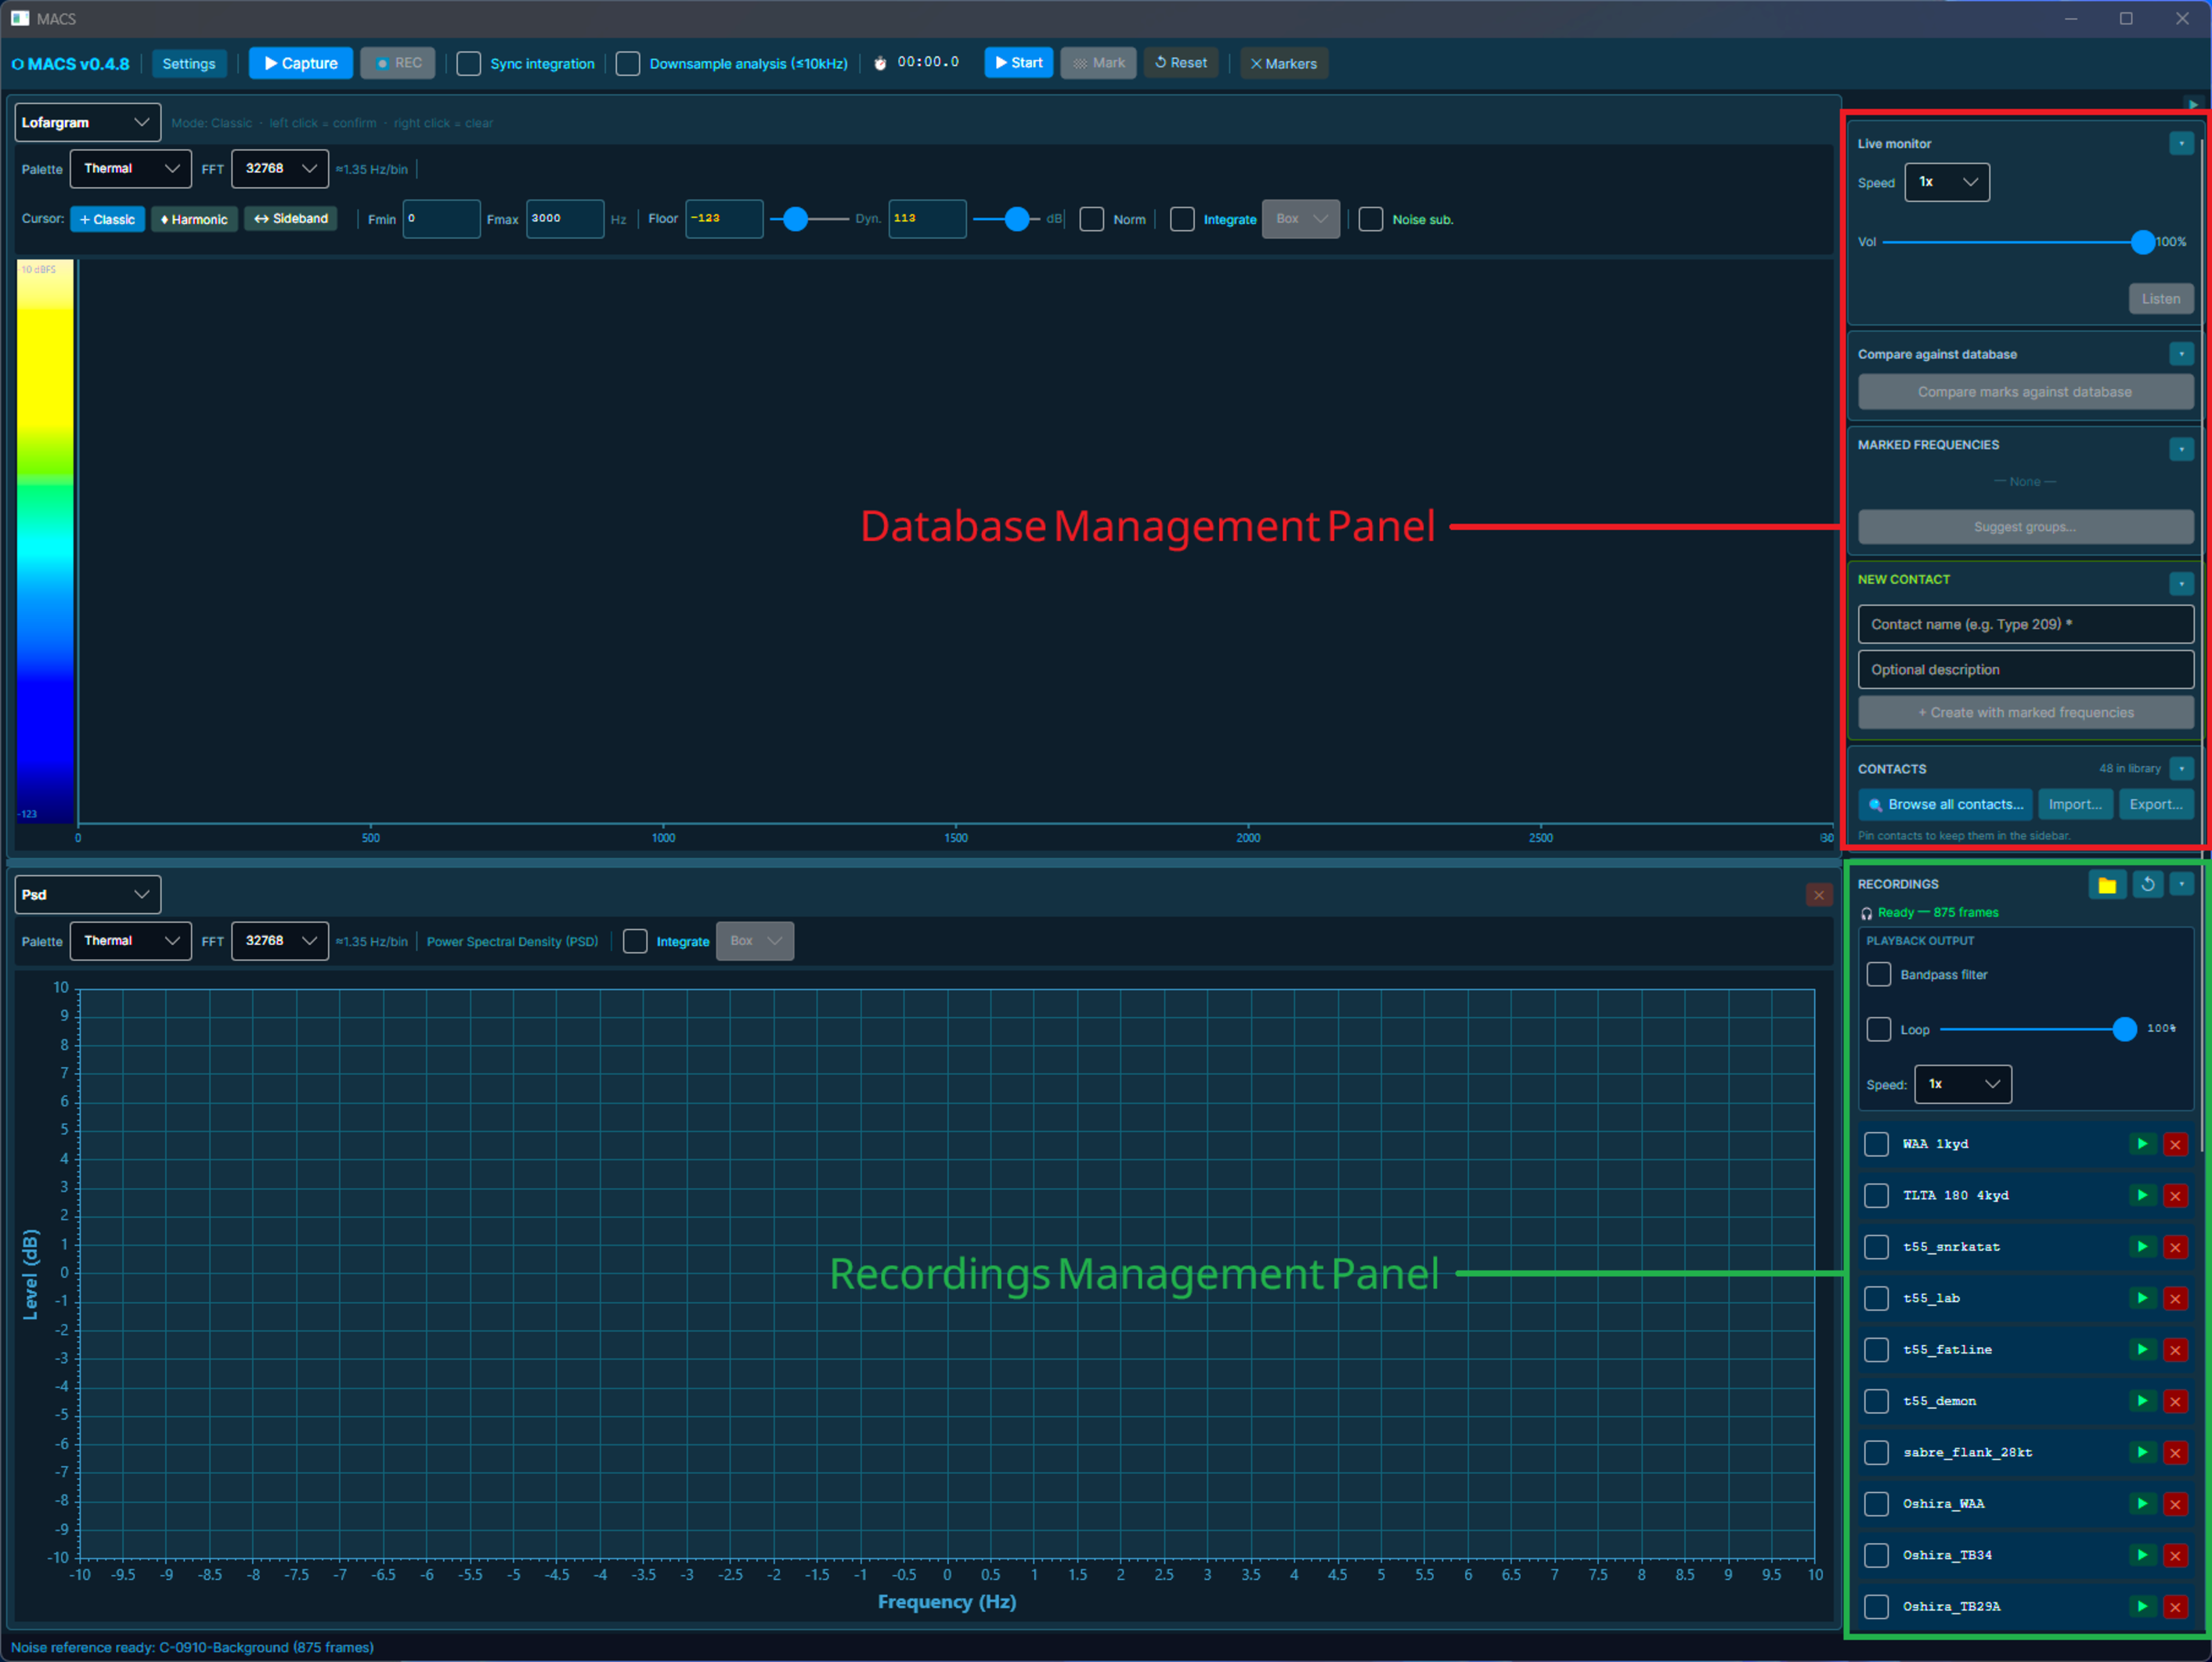
\includegraphics[width=400px]{../img/actuals/MACS_RecordingPanels.pdf}
	\caption{MACS Database and Recordings Panels}
\end{figure}

\subsection{Contact Management}
To browse the contacts in the database, click the \textbf{Browse all contacts} in the \textbf{Contacts} sub-panel Figure 7. This opens the \textbf{Contacts Library} window. Here you can filter the list by entering text in the search box, by tag or by confidence level. The library widow gives you access to the \textbf{Contact Information} panel Figure 8 by clicking either the folder icon or the data icon next to the units name. Both open the same window but at different tabs. The Contact Information window allows you to:

\begin{compactitem}
    \item Enter general information about the contact name, class, nationality, classification confidence etc.
    \item Enter propulsion details, engine type etc.
    \item Ability to set ownship (sets overlay colour to red if checked).
\end{compactitem}

\pagebreak

\begin{figure}[ht]
	\centering
	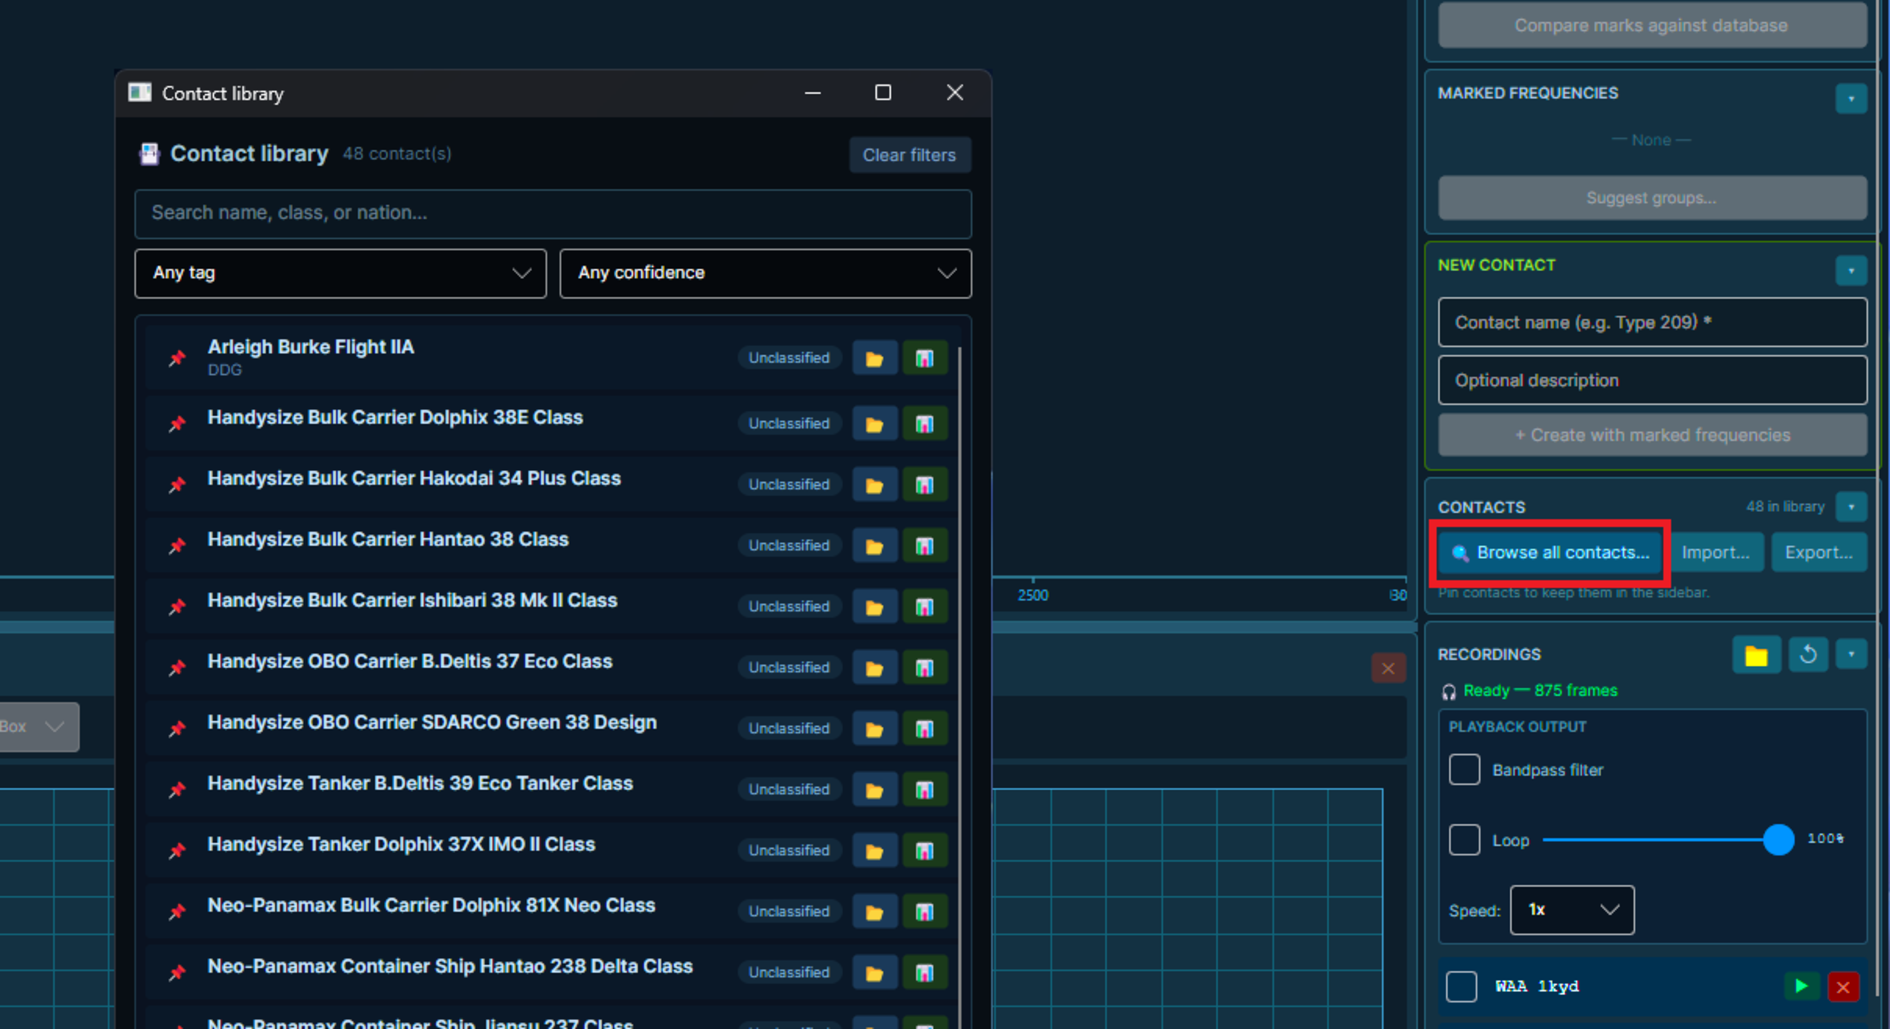
\includegraphics[width=400px]{../img/actuals/BrowseContacts.pdf}
	\caption{Contact Browsing}
\end{figure}

\begin{figure}[ht]
	\centering
	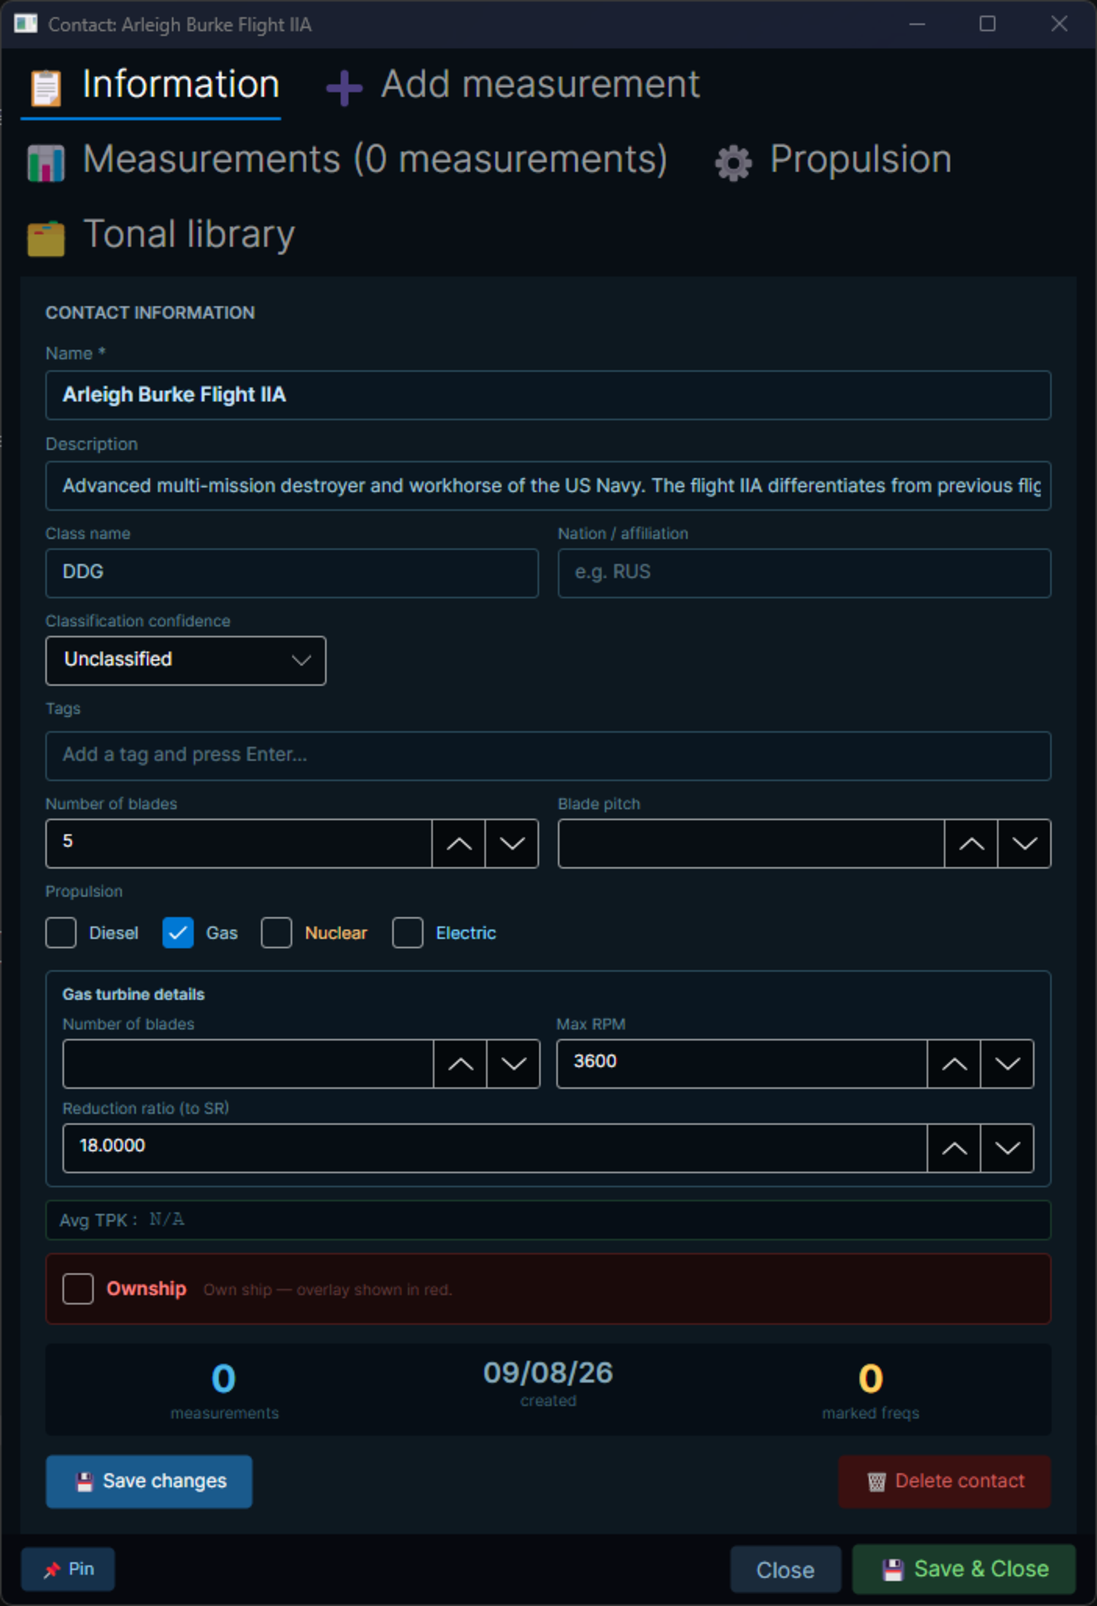
\includegraphics[width=175px]{../img/actuals/MeasurementsPanel.pdf}
	\caption{Measurements Panel}
\end{figure}

\begin{faintquote}
    Note: Saving changes or new measurements requires the user to click the \enquote{\textbf{Save Changes}} button on the left of the panel below the \enquote{\textbf{Ownship}} select box \textbf{before} clicking \enquote{\textbf{Save and Close}}. Just clicking save and close closes the panel without saving the changes.
\end{faintquote}

\subsection{Creating a New Contact}
\textcolor{commentGreen}{*** WIP ***}

To add a new contact at least one frequency must be marked on the LOFARgram (Figure 9). Prominent lines are obvious choices as are the shaft, blade and crankshaft rates. If possible identify the electrical mains and generator set tonals (50 hz or 60hz). These do not slide with speed changes in the same way that some other measures do.

\begin{figure}[ht]
	\centering
	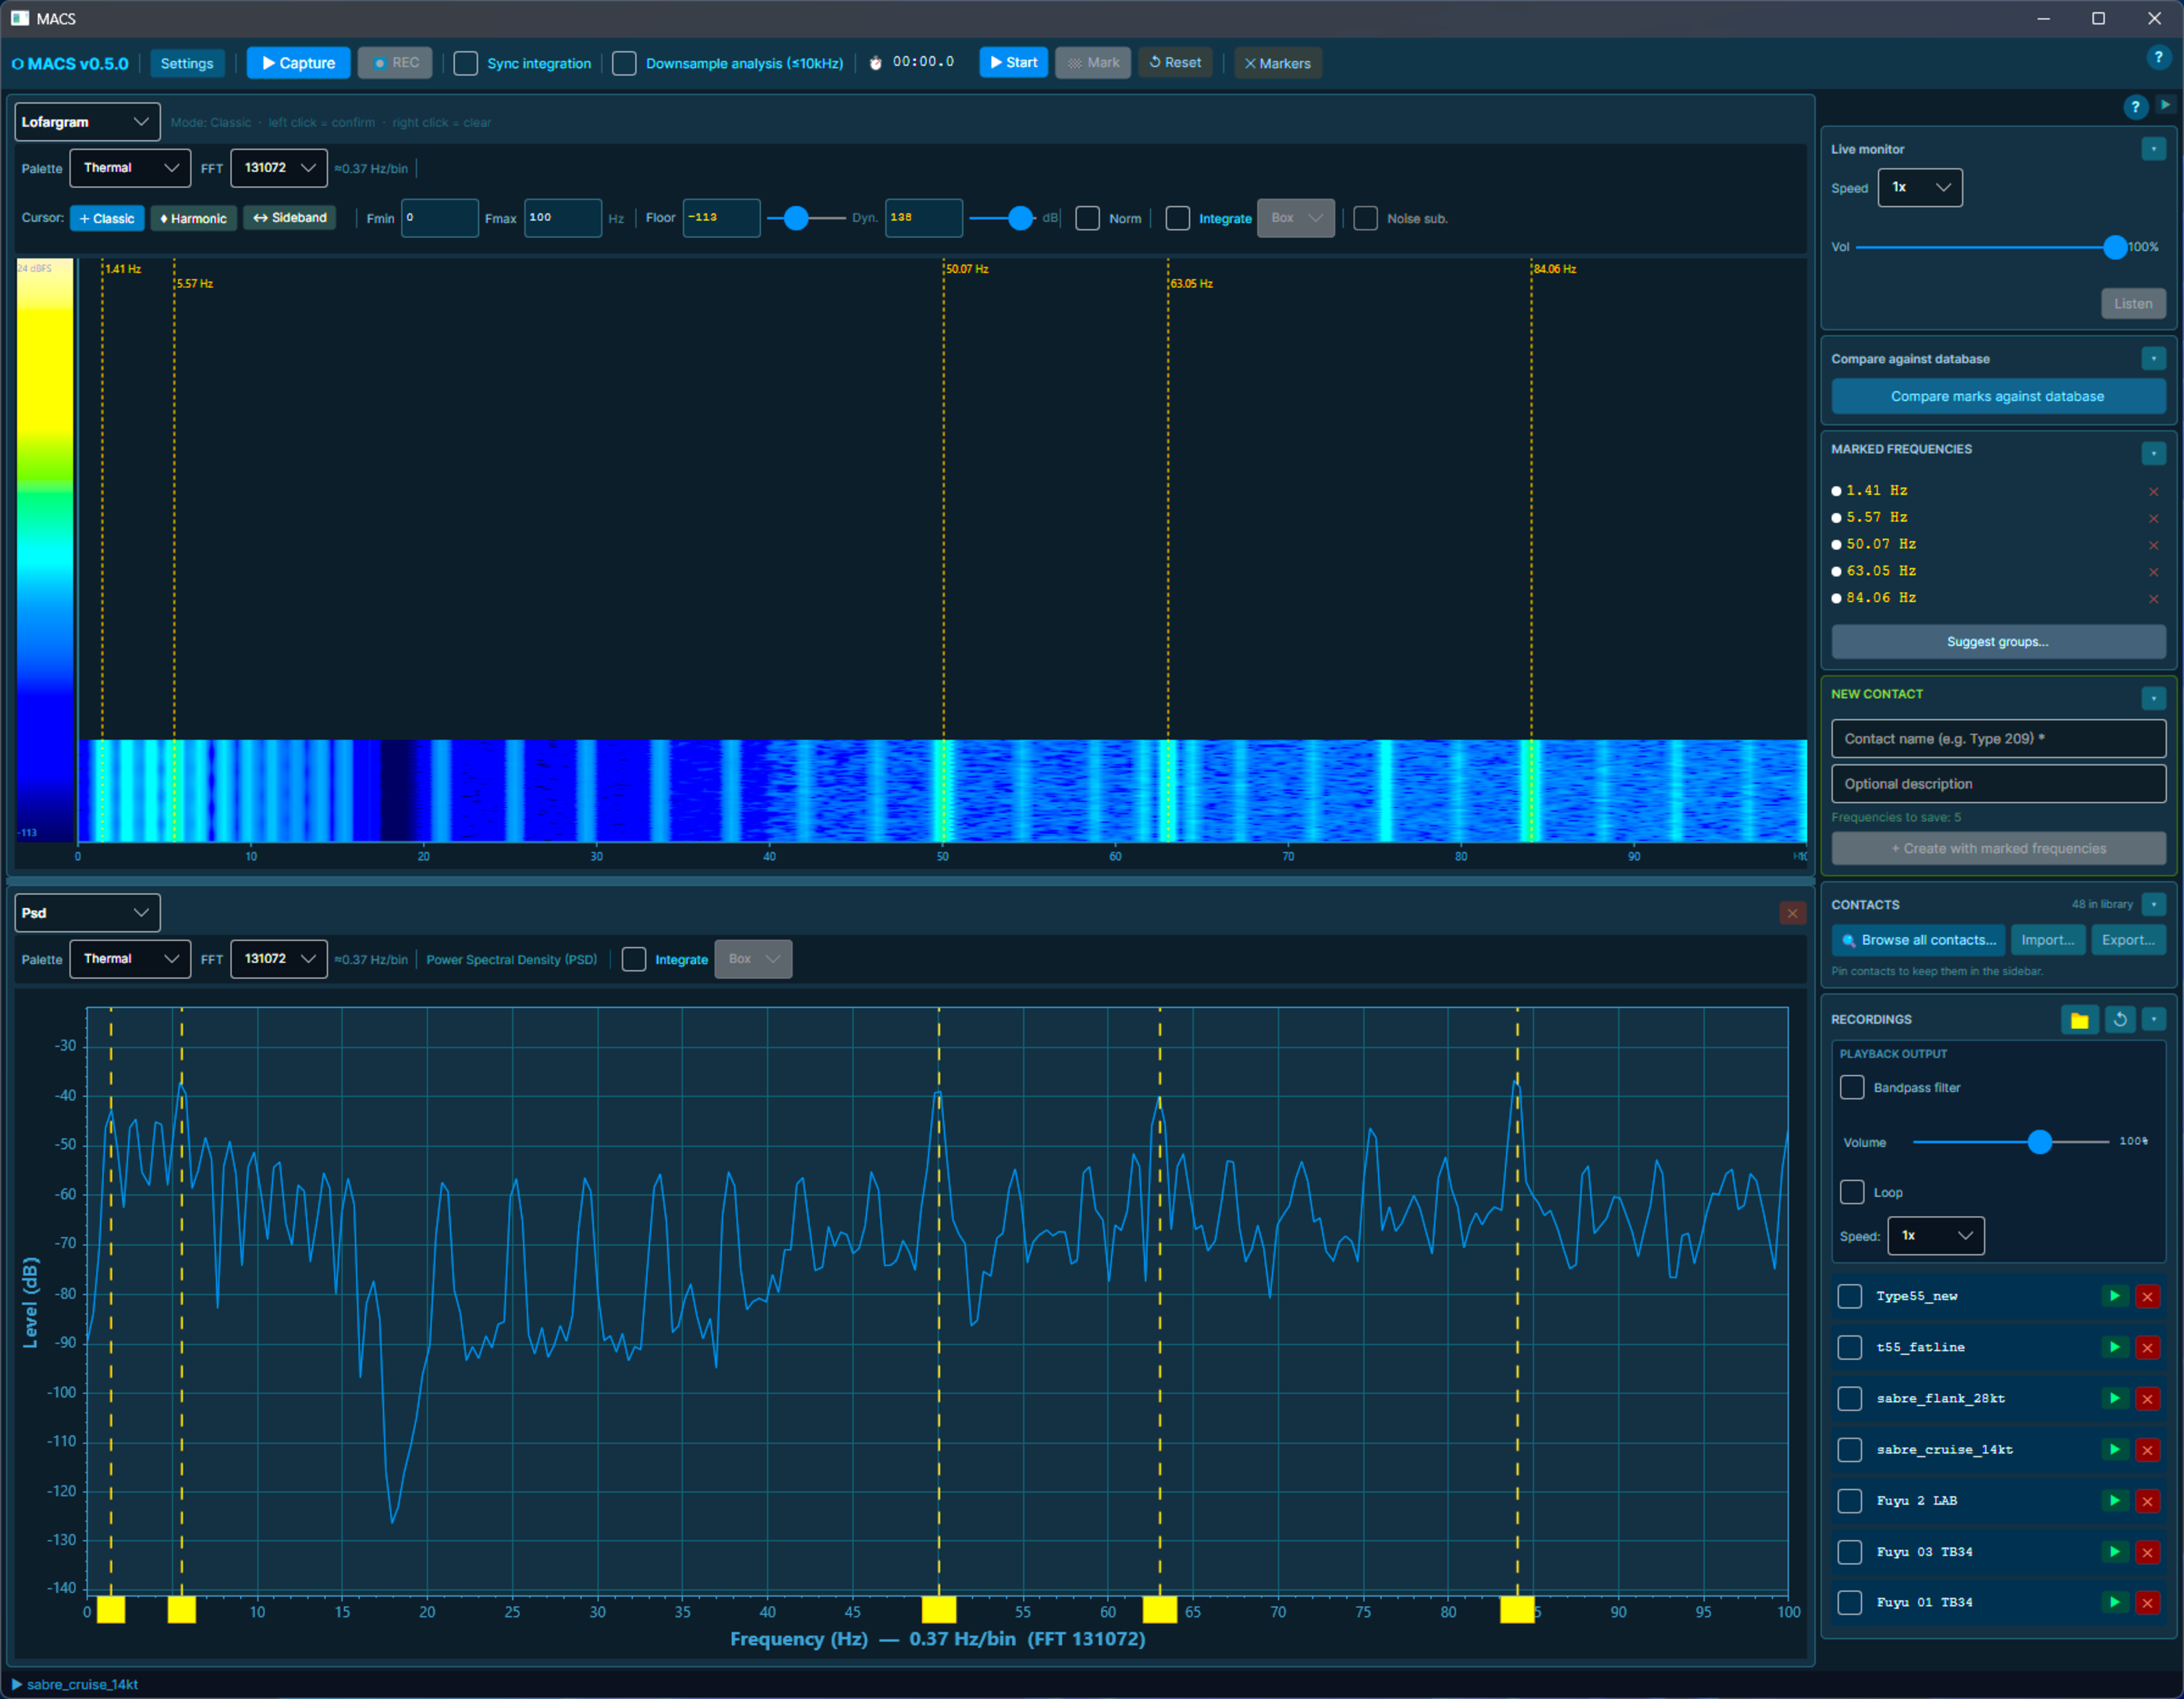
\includegraphics[width=350px]{../img/actuals/Contacts_marked.pdf}
	\caption{Contacts marked on the LOFARgram}
\end{figure}

Before clicking the \enquote{\textbf{+ Create with marked frequencies}} button fill in the \enquote{\textbf{Contact name}} and \enquote{\textbf{Optional description}} fields. On creating the new contact the Measurements Panel (Figure 8) opens where you have the opportunity to add additional measures and refine existing ones. From here you can also capture images of panels A and B for future comparison.

Contact record fields: Information

\begin{compactitem}
    \item Name: Contact identifier (vessel name or designator).
    \item Description.
    \item Class name and nation / affiliation.
    \item Classification confidence, user perception.
    \item Tag, add a tag to aid future identification, user setting
    \item Blade count: Number of propeller blades.
    \item Blade pitch: Pitch of propeller blades.
    \item Propulsion type, each checkbox opens a sub-panel allowing further detail entry
    \item Ownship when selected identifies this contact as ownship
\end{compactitem}

Contact record fields: Add measurement
\begin{compactitem}
    \item Advanced editor opens the Advanced Tonal Editor panel.
    \item Estimated speed (knots) user enters their estimations of target speed (optional)
    \item Estimated Distance (m) users distance estimation (optional)
    \item Shaft Rate (SR): Propeller shaft rotation rate in rev/s (Hz).
    \item Crankshaft Rate (CSR): Engine crankshaft rate in rev/s.
    \item Reduction factor - auto-computed $CSR / SR$. The gear reduction between engine and shaft.
    \item TPK: Turns Per Knot - auto-computed (see below). Indicates how many shaft revolutions per knot of speed.
    \item Frequency overlays: Named sets of frequency markers from the LOFARgram.
\end{compactitem}

TPK (Turns Per Knot) is computed as:

\[
TPK = \frac{SR \times 60}{Speed}
\]

This gives shaft turns per knot of vessel speed, which is a vessel-class characteristic independent of operating condition. Average TPK is computed across all measurements for a contact and shown in the contact list for quick comparison. Refinements to this calculation which include such factors as slippage are discussed in Appendix C.

The \enquote{\textbf{Measurements (n measurements)}}, \enquote{\textbf{Propulsion}} and \enquote{\textbf{Tonal library}} give access to visual representations of the contacts measurements.

To complete the process scroll to the bottom of the measurements panel and click the \enquote{\textbf{"+ Save this measurement"}} button before saving and closing the panel.

To add a measurement to an existing contact, navigate to the measurements panel (page 18) and select the \enquote{\textbf{+ Add measurement}} tab. Enter the details and then click the \enquote{\textbf{+ Save this measurement}} button before saving and closing.

\subsubsection{Advanced Tonal Editor panel and Grouping}
\textcolor{commentGreen}{*** WIP ***}

\subsubsection{Overlays}
\textcolor{commentGreen}{*** WIP May Not Be Needed ***}

Overlays let you annotate the LOFARgram with frequency markers that are saved to the contact database.

Overlay controls

\begin{compactitem}
    \item \textbf{New overlay:} Creates a new named overlay (associated with a contact).
    \item \textbf{Colour picker:} Sets the display colour for the selected overlay.
    \item \textbf{Error band:} Adds $\pm$ frequency uncertainty bars around each marker.
    \item \textbf{Line width:} Controls marker line thickness in pixels.
    \item \textbf{Cursor mode colouring:} Colours each line by the cursor mode that created it (Single /Harmonic /Resonance each get a distinct colour), overriding the overlay colour.
\end{compactitem}

Each frequency point stores its Hz value and the cursor mode used to capture it. This means the database records not just where the line is, but how it was identified: as a single tonal, a harmonic fundamental, or a resonance line.

\subsection{Contact Matching}
\textcolor{commentGreen}{*** WIP ***}

The central purpose of the database is to enable the user to classify and, potentially identify, an unknown contact. It stands to reason that in order to do this the user must have added contacts and measures to the database in order for the matching system to work.

The basic workflow is:

\begin{compactenum}
    \item For your unknown contact mark significant tonals, for instance, but not exclusively: SR, BR, CSR and electrical mains.
    \item Click the \enquote{\textbf{Compare marks against database}} in the compare against database sub-panel.
    \item In the \enquote{\textbf{Comparison results}} panel enter any additional information you may have in the \enquote{\textbf{Target known details}} fields (Figure 10 - Green Boxes).
    \item If no matches reach the partial or pass criteria adjust the tolerance setting to allow for variation in accuracy in placing markers. Too broad a tolerance will cause more misidentifications which will have to be discounted by observation (Figure 10 - Red Box)
    \item In an ideal situation you will end up with a single match (Figure 11) although it is more likely that you will have more than one and several partials.
\end{compactenum}

\begin{faintquote}
    The contact database has a lot of hidden content and features, this section is a quick overview of the functionality offered. A detailed walk through of creating, managing and matching contacts is given in the Illustrated Examples section.
\end{faintquote}

\begin{figure}[ht]
	\centering
	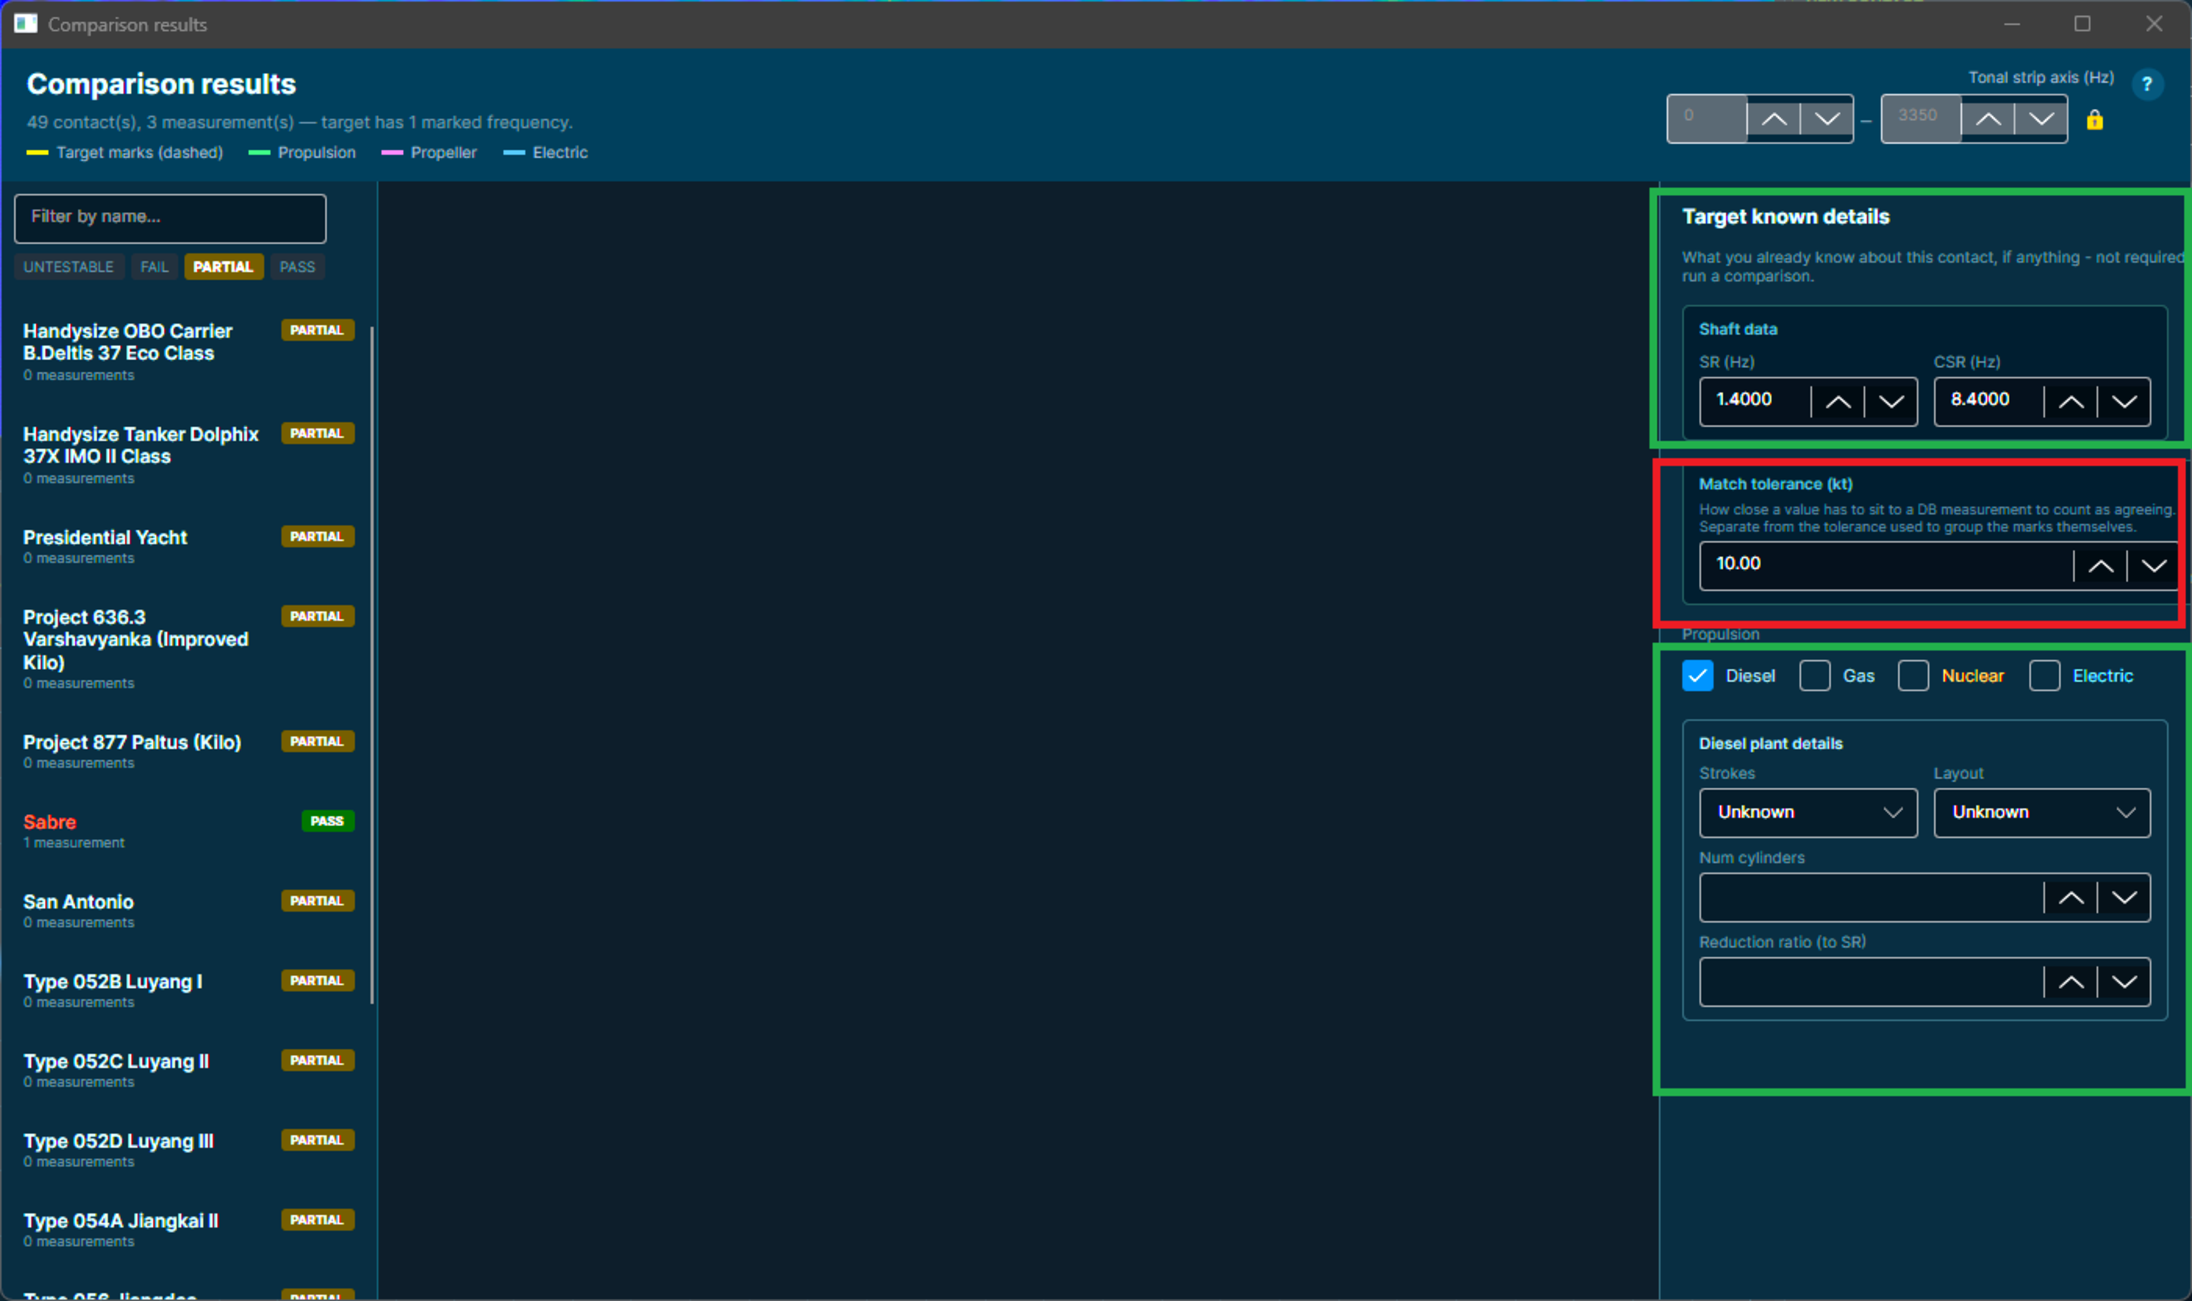
\includegraphics[width=350px]{../img/actuals/Contact_01.pdf}
	\caption{Partial Contacts}
\end{figure}

\begin{figure}[ht]
	\centering
	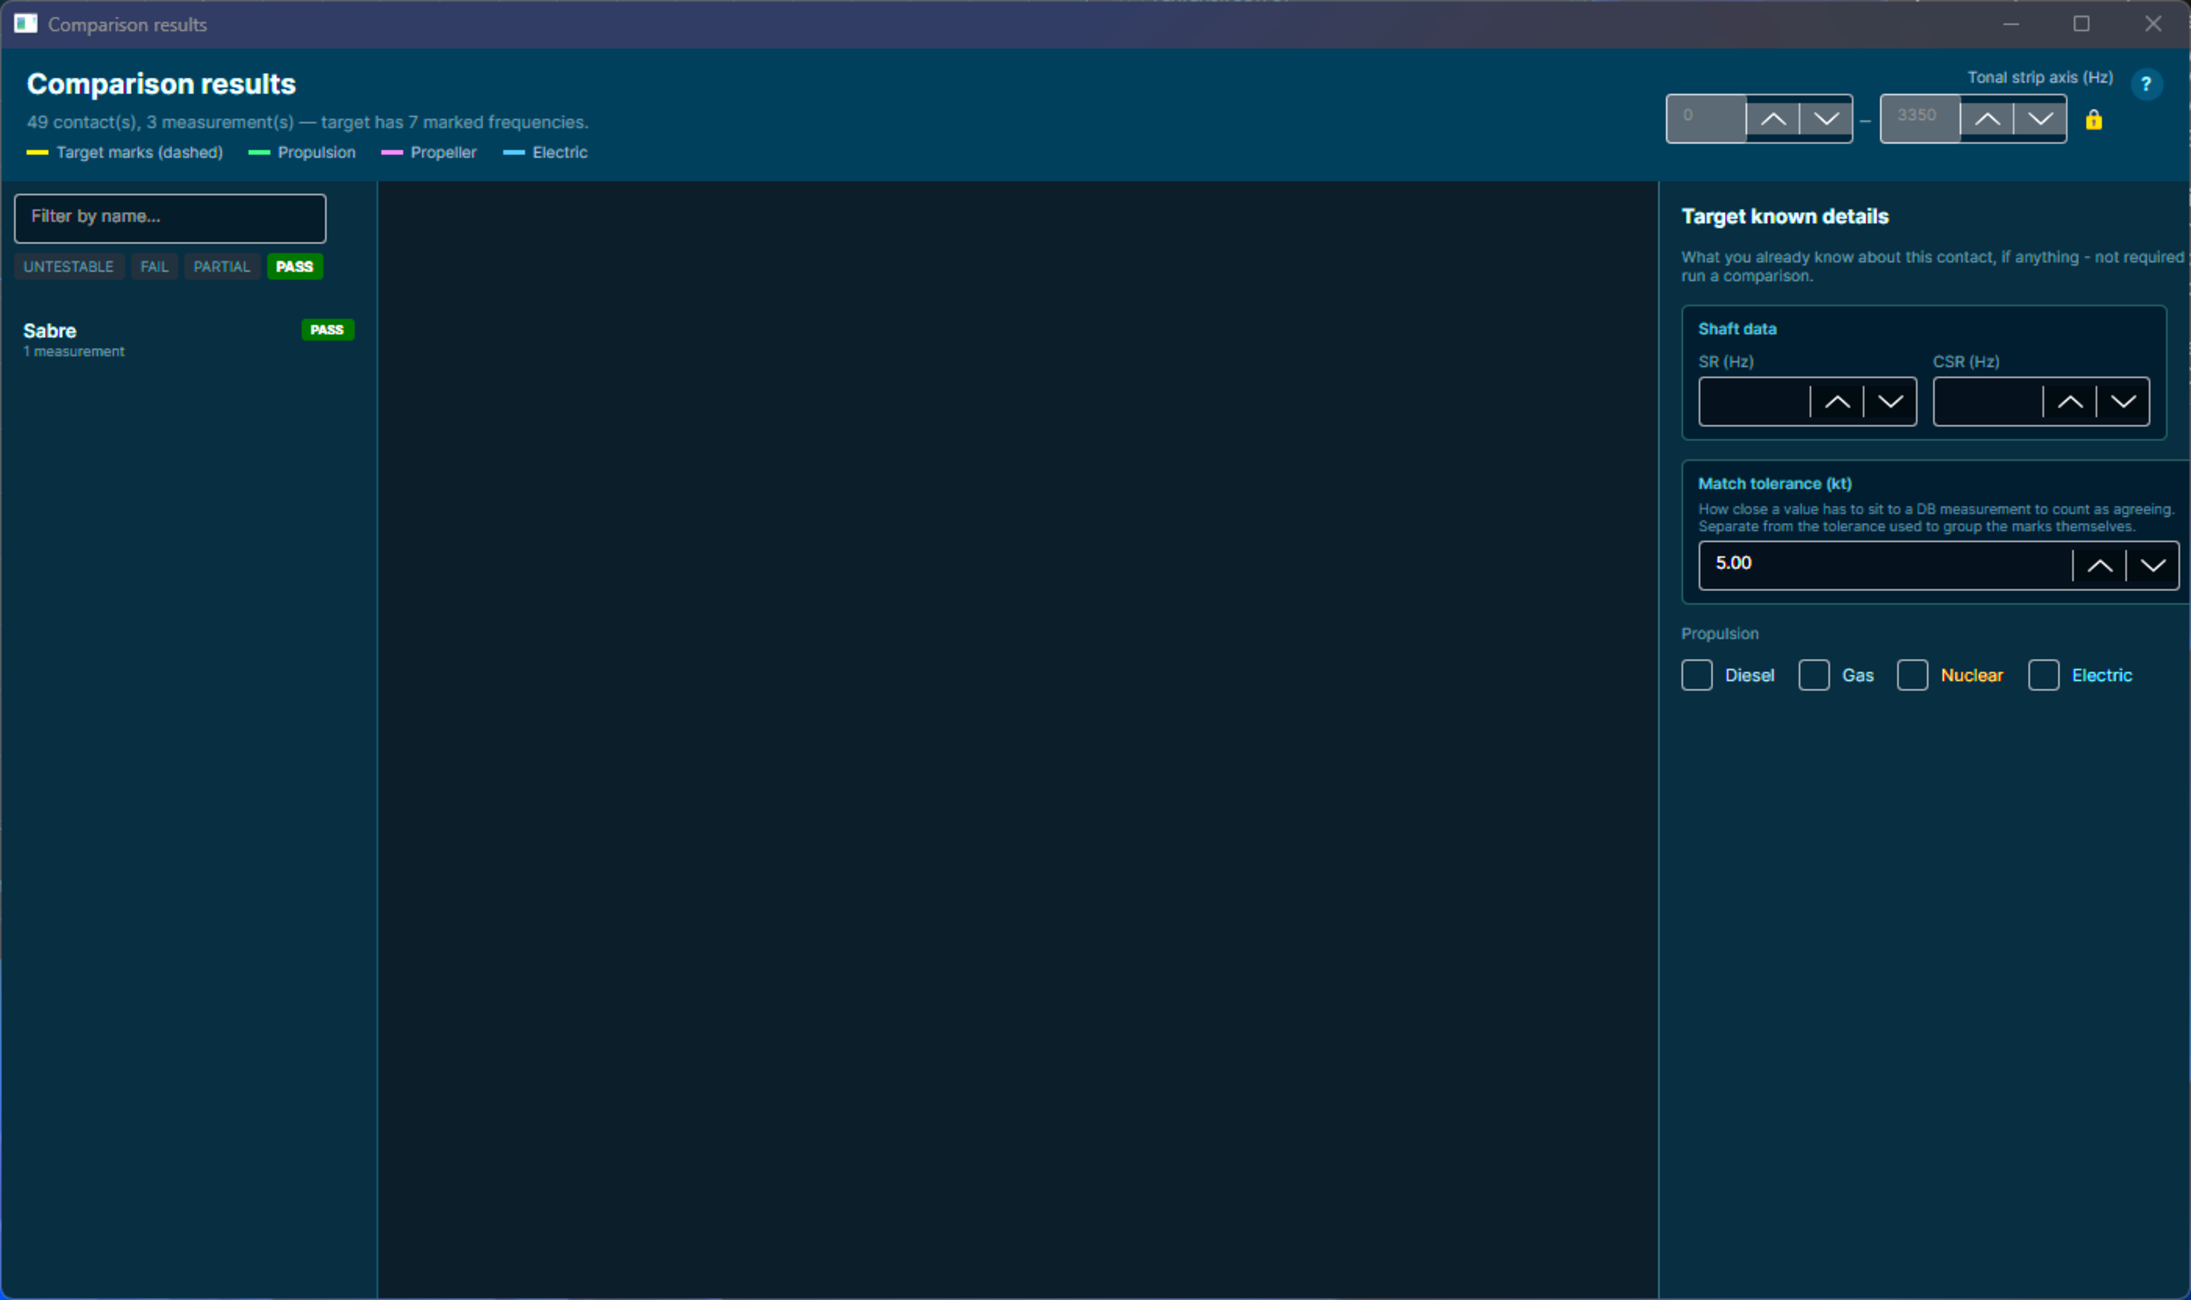
\includegraphics[width=350px]{../img/actuals/Contact_02.pdf}
	\caption{A Single Match}
\end{figure}

\subsubsection{Live Monitor}
\textcolor{commentGreen}{*** WIP ***}

%\FloatBarrier
%\pagebreak
\clearpage